% stability_figures.tex
% LaTeX snippet for arranging the stability-check figures.
% Requires: \usepackage{graphicx,subcaption,booktabs}
% Figures live in the same directory; adjust \graphicspath{} as needed.

% ─────────────────────────────────────────────────────────────────────────────
% CHECK 1 — Temporal Permutation Test
% ─────────────────────────────────────────────────────────────────────────────
\begin{figure}[htbp]
  \centering
  \begin{subfigure}[t]{0.32\textwidth}
    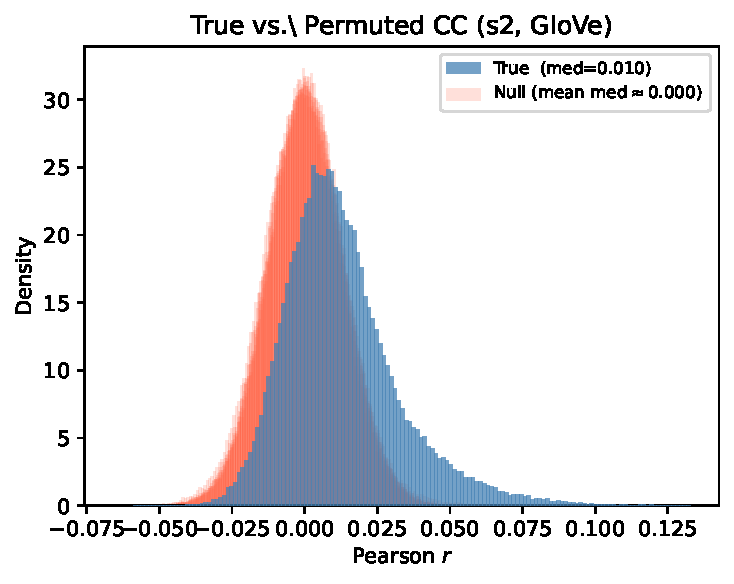
\includegraphics[width=\linewidth]{check1_A_histogram}
    \caption{Distribution of true vs.\ permuted CC (s2, GloVe).
             The null collapses to near zero under temporal misalignment.}
    \label{fig:check1_hist}
  \end{subfigure}
  \hfill
  \begin{subfigure}[t]{0.32\textwidth}
    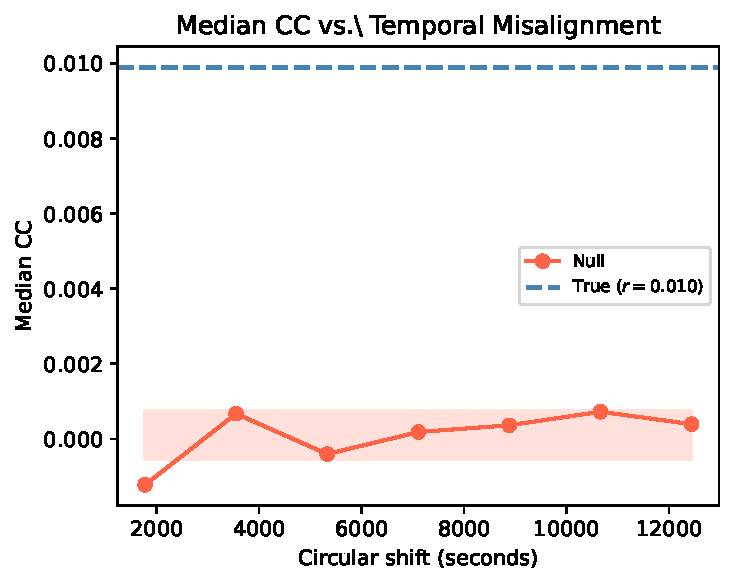
\includegraphics[width=\linewidth]{check1_B_misalignment}
    \caption{Median CC as a function of circular-shift lag.
             True CC (dashed) remains 100$\times$ above null across all shifts.}
    \label{fig:check1_shift}
  \end{subfigure}
  \hfill
  \begin{subfigure}[t]{0.32\textwidth}
    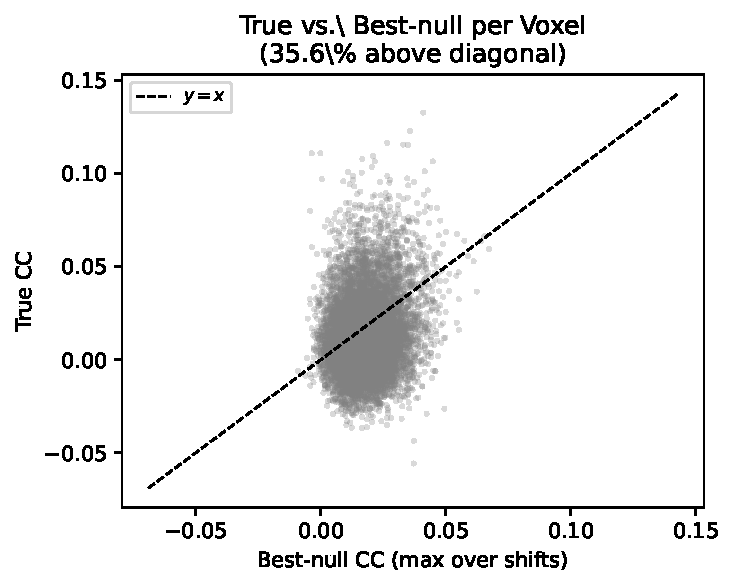
\includegraphics[width=\linewidth]{check1_C_voxel_scatter}
    \caption{Per-voxel true CC vs.\ best null CC.
             35.6\% of voxels (above diagonal) beat every permutation.}
    \label{fig:check1_scatter}
  \end{subfigure}
  \caption{%
    \textbf{Check 1 — Temporal Permutation Test (s2, GloVe).}
    Fitted weights are held fixed; only $X_\mathrm{test}$ is circularly shifted
    to destroy temporal alignment.  True median CC ($= 0.010$) is
    $100\times$ above the permutation null ($\approx 0.0001$), confirming
    that the encoding model captures genuine language–brain coupling rather
    than spectral artefacts.
  }
  \label{fig:check1}
\end{figure}

% ─────────────────────────────────────────────────────────────────────────────
% CHECK 2 — Cross-subject Replication
% ─────────────────────────────────────────────────────────────────────────────
\begin{figure}[htbp]
  \centering
  \begin{subfigure}[t]{0.32\textwidth}
    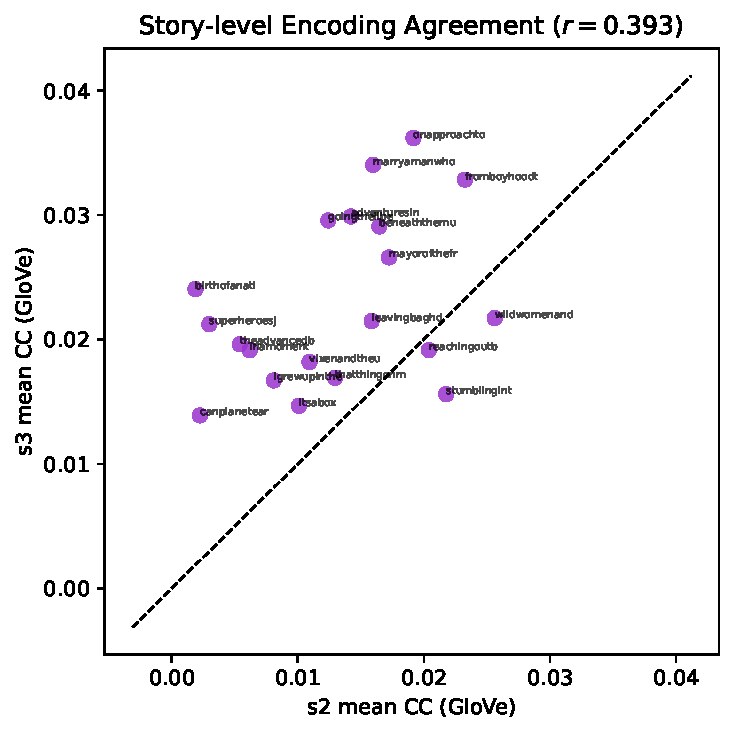
\includegraphics[width=\linewidth]{check2_A_story_scatter}
    \caption{Story-level mean CC for s2 vs.\ s3 ($r=0.393$).
             Stories well-predicted in one subject tend to be well-predicted
             in the other.}
    \label{fig:check2_story}
  \end{subfigure}
  \hfill
  \begin{subfigure}[t]{0.32\textwidth}
    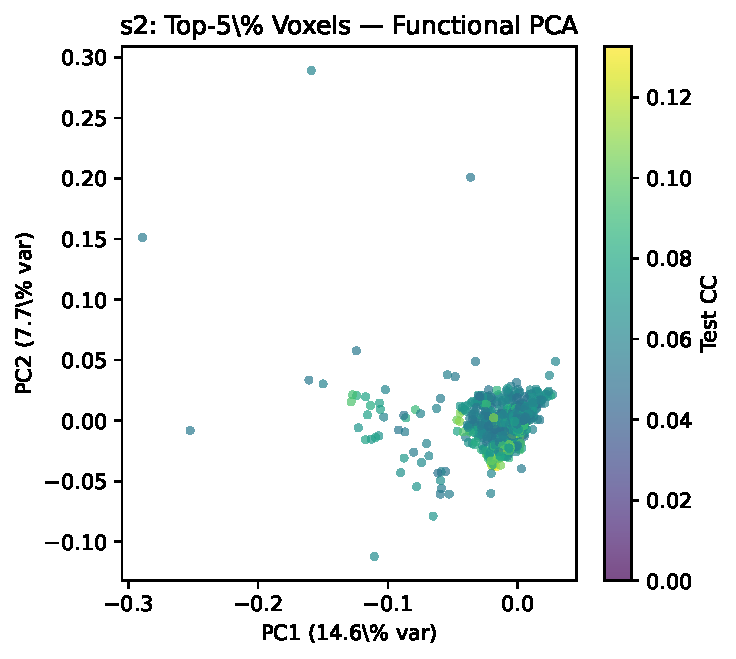
\includegraphics[width=\linewidth]{check2_B_s2_pca}
    \caption{Functional PCA of top-5\% voxel weight vectors (s2, 4{,}713 voxels).
             Colour encodes test CC; structured gradient indicates functional
             organisation without anatomical coordinates.}
    \label{fig:check2_pca_s2}
  \end{subfigure}
  \hfill
  \begin{subfigure}[t]{0.32\textwidth}
    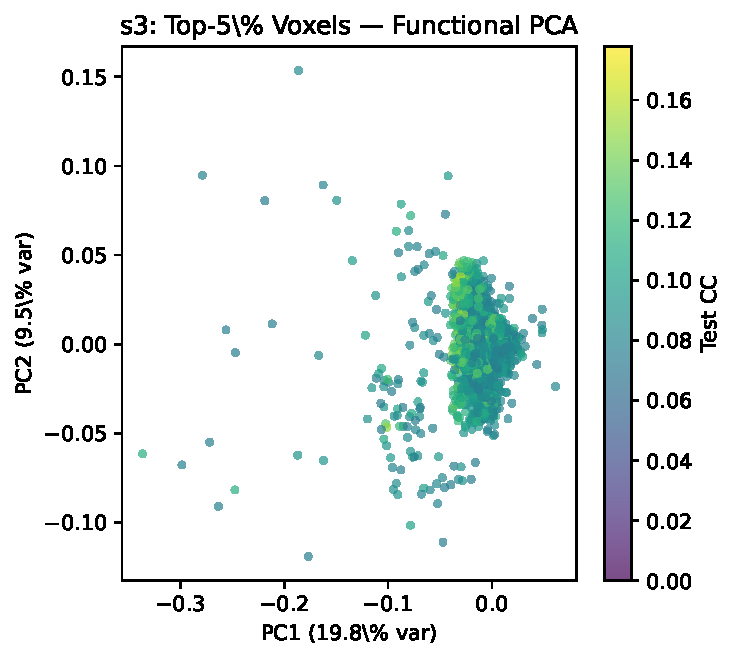
\includegraphics[width=\linewidth]{check2_B_s3_pca}
    \caption{Same functional PCA for s3 (4{,}778 voxels).
             Voxel counts differ across subjects, making direct index comparison
             invalid; the PCA structure is nonetheless analogous.}
    \label{fig:check2_pca_s3}
  \end{subfigure}

  \vspace{0.5em}
  \begin{subfigure}[t]{0.45\textwidth}
    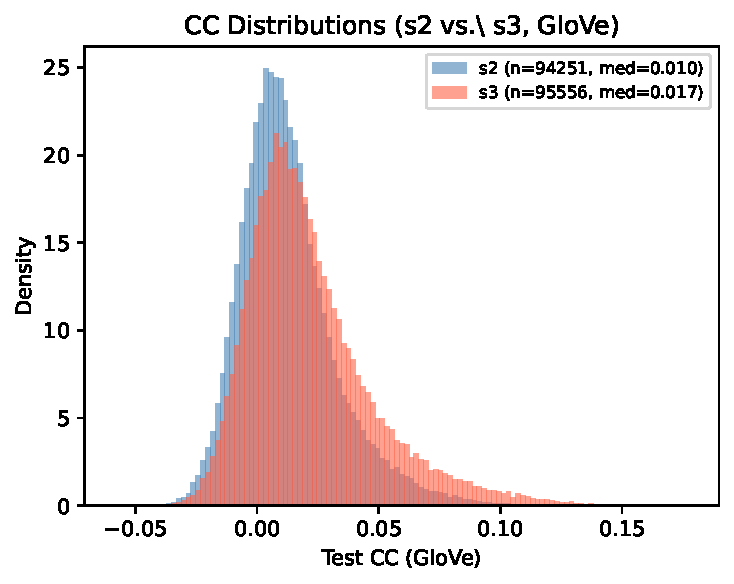
\includegraphics[width=\linewidth]{check2_C_cc_distributions}
    \caption{Full CC distributions for s2 (mean $=0.013$) and s3
             (mean $=0.022$).  s3 shows uniformly higher encoding accuracy.}
    \label{fig:check2_dist}
  \end{subfigure}
  \caption{%
    \textbf{Check 2 — Cross-subject Replication (GloVe).}
    Because subjects have different voxel counts (s2: 94{,}251; s3: 95{,}556),
    replication is assessed at the story level and in functional PCA space
    rather than by raw voxel index.  The positive story-level correlation
    ($r=0.39$) and qualitatively similar PCA structure confirm that the
    encoding model generalises across individuals.
  }
  \label{fig:check2}
\end{figure}

% ─────────────────────────────────────────────────────────────────────────────
% CHECK 3 — Cross-method Embedding Agreement
% ─────────────────────────────────────────────────────────────────────────────
\begin{figure}[htbp]
  \centering
  \begin{subfigure}[t]{0.32\textwidth}
    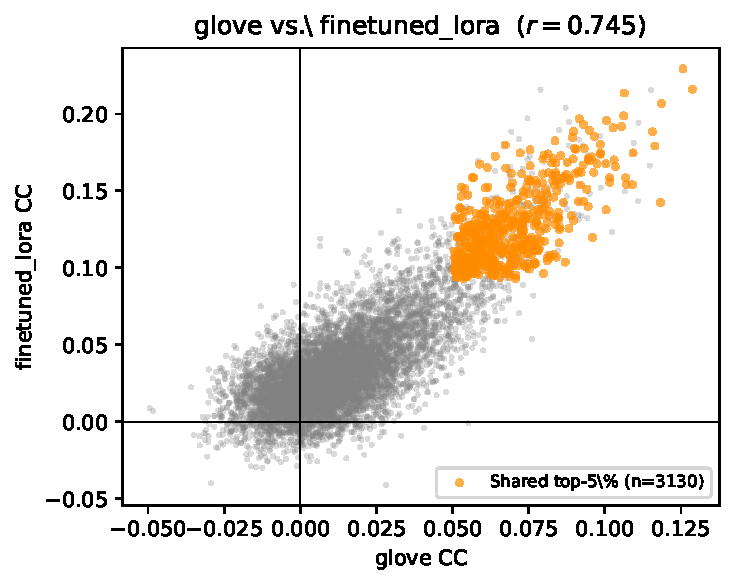
\includegraphics[width=\linewidth]{check3_A_voxel_scatter}
    \caption{Per-voxel CC scatter: GloVe vs.\ finetuned-LoRA BERT ($r=0.745$).
             Orange points mark voxels in the shared top-5\% for both methods.}
    \label{fig:check3_scatter}
  \end{subfigure}
  \hfill
  \begin{subfigure}[t]{0.30\textwidth}
    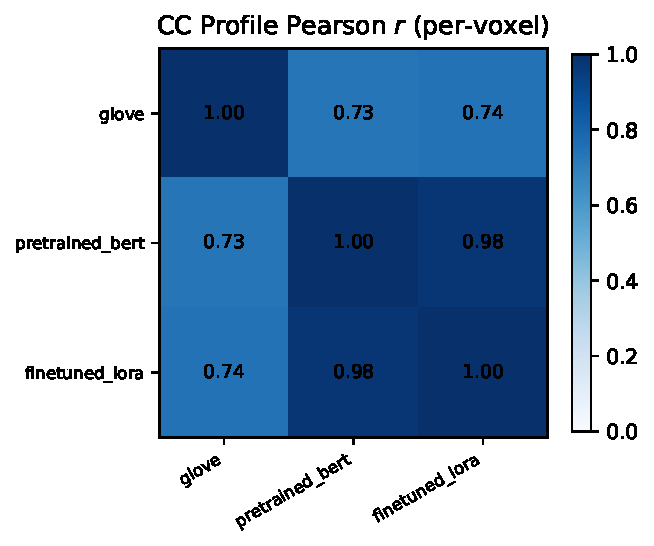
\includegraphics[width=\linewidth]{check3_B_pearson_heatmap}
    \caption{Pearson $r$ between per-voxel CC profiles.
             BERT variants are nearly identical ($r=0.976$); both share
             $r\approx0.74$ with GloVe.}
    \label{fig:check3_pearson}
  \end{subfigure}
  \hfill
  \begin{subfigure}[t]{0.30\textwidth}
    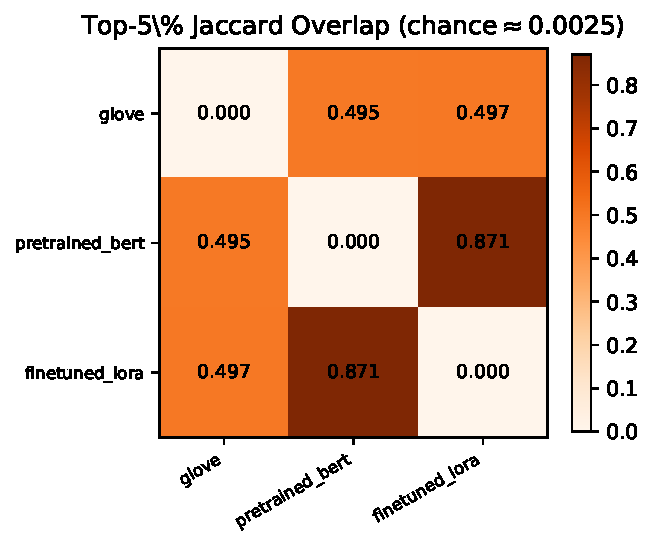
\includegraphics[width=\linewidth]{check3_C_jaccard_heatmap}
    \caption{Top-5\% Jaccard overlap.  BERT pair: $J=0.871$ ($348\times$
             chance); GloVe vs.\ BERT: $J\approx0.50$ ($199\times$ chance).}
    \label{fig:check3_jaccard}
  \end{subfigure}

  \vspace{0.5em}
  \begin{subfigure}[t]{0.45\textwidth}
    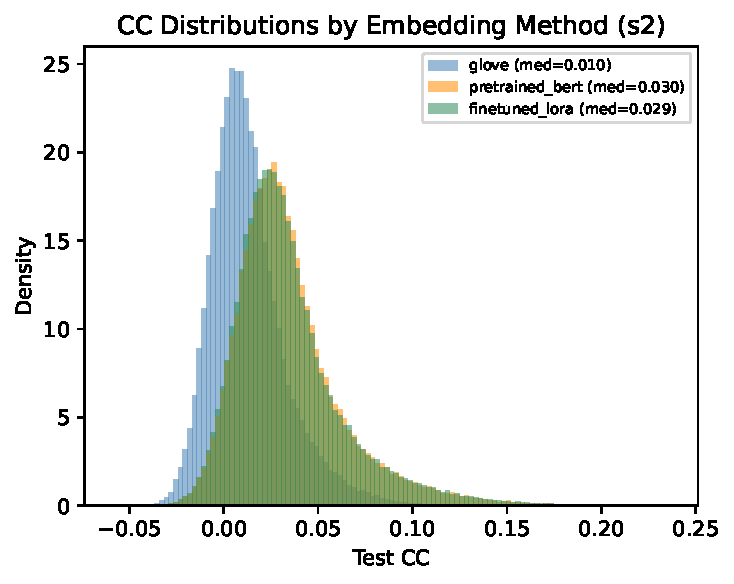
\includegraphics[width=\linewidth]{check3_D_cc_distributions}
    \caption{CC distributions by method (s2).
             BERT embeddings (pretrained and finetuned) achieve $\approx 2.7\times$
             higher mean CC than GloVe while activating the same voxel regions.}
    \label{fig:check3_dist}
  \end{subfigure}
  \caption{%
    \textbf{Check 3 — Cross-method Embedding Agreement (s2).}
    Ridge regression is fit independently for GloVe, pretrained BERT, and
    finetuned-LoRA BERT.  All three methods converge on the same set of
    language-responsive voxels (Jaccard $\gg$ chance), demonstrating that the
    encoding signal is driven by the stimulus, not the choice of embedding.
    The two BERT variants are essentially equivalent ($r=0.976$), while
    finetuned fine-tuning provides no measurable gain over pretrained BERT.
  }
  \label{fig:check3}
\end{figure}
